\documentclass{TDP003mall}



\newcommand{\version}{Version 1.0}
\author{Nils Bark, \url{nilba048@student.liu.se}\\
  Hadi Ansari, \url{hadan326@student.liu.se}}
\title{Dokumentmall}
\date{2020-12-07}
\rhead{Nils Bark\\
Hadi Ansari}



\begin{document}
\projectpage
\section{Revisionshistorik}
\begin{table}[!h]
\begin{tabularx}{\linewidth}{|l|X|l|}
\hline
Ver. & Revisionsbeskrivning & Datum \\\hline
0.1 & Första utkast skapat & 2020-11-27\\\hline
1.0 & Uppdatering av utkast enligt feedback från handledare & 2020-12-07\\\hline
\end{tabularx}
\end{table}

\section{Beskrivning av Entity}
Nedan kommer en lista över alla funktioner och variabler som finns i klassen \texttt{Entity}.
\subsection{Variabler}
\begin{itemize}
\item \texttt{sf::Vector2f location}: Innehåller två koordinater av typen float som representerar spelarens position på spelplanen.
\item \texttt{sf::Texture texture}: Tar in en bild och använder den som textur för ett objekt.
\item \texttt{sf::Sprite sprite}: Fungerar som figurens kropp och kan täckas av en textur.
\item \texttt{float speed}: Används för att bestämma objekts hastighet. 
\item \texttt{int health}: Bestämmer objektets livspoäng.
\item \texttt{int width och int height}: Bestämmer objektets storlek.

\end{itemize}
\subsection{Funktioner}
\begin{itemize}
\item \texttt{virtual void Tick(sf::Time const \& delta) = 0}: Uppdaterar objektens position. Den implementeras av de härledda klasserna och beteer sig där på olika sätt. 
Till exempel för Big plane så subtraheras x-koordinaten med ett värde som är bundet till hastigheten och tiden som har gått sedan förra uppdateringen.
\item \texttt{virtual bool Want\_shoot() = 0}: Returnerar true om objektet vill skjuta, annars false. Till exempel returneras alltid false för bomber eftersom de aldrig skjuter, 
medan true returneras när spelaren trycker ned mellanslag (om andra faktorer tillåter).
\item \texttt{virtual Entity* shoot() = 0}: Returnerar en entity-pekare som pekar på \texttt{player\_bullet} eller \texttt{enemy\_bullet} beroende på om det är spelaren eller en fiende som ska skjuta. 
Har ingen definition i klasser som aldrig kommer att använda shoot().
\item \texttt{bool kill\_me()}: Kontrollerar om ett objekt ska förstöras (till exempel om det befinner sig utanför spelplanen) och returnerar true om så är fallet.
\item \texttt{virtual void collision(vector<entity*> objects) = 0}: Tar en lista som inehåller entity-pekare till alla andra spelobjekt, utöver det som kallat på funktionen, 
och kontrollerar vilket av  dem objektet har kolliderat med. Har flera olika effekter beroende på vilket objekt som har kolliderat med ett annat. Till exempel förlorar spelaren liv om den kolliderar med en fiende. 
\item \texttt{virtual string get\_type() = 0}: Returnerar objektets typ i form av en sträng. 
\end{itemize}

\texttt{Entity} är en \texttt{abstract struct} som alla understående klasser i spelet ärver ifrån. Detta innebär att alla dess variabler och funktioner är tillgängliga direkt i de härledda klasserna.
\texttt{Entity} låter oss därmed uppdatera alla andra objekt i spelet. 
Detta sker via funktionen \texttt{tick()} som tar in en parameter av typen \texttt{sf::Time} och uppdaterar positionen för alla objekt på skärmen. 
\texttt{Tick()} är en \texttt{virtual} funktion som kan överskrivas i de härledda klasserna.
Tack vare tidsberäkningen som sker innuti funktionen är vi oberoende av spelets bildfrekvens och tiden det tar att hantera alla händelser i loopen.
Alla datamedlemmar förutom \texttt{location} i basklassen kommer att initieras av de härledda klassernas constructor. 
till exempel kommer spelarens \texttt{speed} att initieras när spelaren skapas och inte innan.

\section{Beskrivning av Player}
Nedan kommer en lista över alla funktioner och variabler som finns i klassen \texttt{Player}.
\subsection{Variabler}
\begin{itemize}
\item \texttt{bool sht}: Är true då spelaren trycker på mellanslag (och därmed vill skjuta), false annars.
\item \texttt{float shoot\_speed}: Bestämmer tiden som måste passera efter att spelaren har skjutit innan den får skjuta igen.
\item \texttt{sf::Clock clock1}: Är en klocka som mäter tiden som har gått mellan spelarens skott.
\item \texttt{sf::Time t1}: Sparar tiden som har passerat enligt clock1 i form av sekunder.
\item \texttt{bool shield}: Är true om spelaren har shield-effekten aktiv.
\item \texttt{sf::Clock shield\_clock}: Räknar tiden från och med att spelaren plockade upp en shield-powerup
\end{itemize}

\subsection{Funktioner}
\begin{itemize}
\item \texttt{sf::Vector2f process\_event(sf::Time delta)}: Hanterar händelser åt spelaren. Till exempel vilka tangenter som trycks ner och vad som då ska hända.
\item \texttt{string get\_shield\_time()}: Returnerar den kvarstående tiden från \texttt{shield\_clock}.
\item \texttt{bool has\_shield()}: Returnerar true om spelaren har en shield aktiv, annars false.
\end{itemize}

\texttt{Player} representerar det objekt som användaren kommer att ha kontroll över under spelets gång. 
Det är en härledd klass av \texttt{Entity} och ärver därmed alla datamedlemmar och funktioner därifrån. 
Den har också en känna-till-relation till \texttt{player\_bullet} och \texttt{Power-ups} härledda klasser.
Player använder sig av process\_event för att uppdatera \texttt{sht} (ifall det tillåts av de andra faktorerna)  eller uppdatera spelarens \texttt{location}. 
Player överskriver \texttt{tick()} för att kunna läsa in en ny \texttt{location} som \texttt{process\_event()} har uppdaterat och sätta spelarens position baserat på det.
Förutom de variabler den ärver har \texttt{Player} även en \texttt{int health} som avgör spelarens liv. 
I spelarens konstruktor initieras spelarens \texttt{health, location, speed, shoot\_speed, sht, t1, shield, sprite} och \texttt{texture}.
\texttt{kill\_me()} kollar här om spelarens liv hamnar på eller under 0. Om detta händer förstörs spelaren och spelet är över.

Spelarens kollision med andra objekt kontrollerar ständigt under spelets gång via \texttt{collision()} från \texttt{entity}. Baserat på vilket objekt som spelaren kolliderar med kan flera olika saker hända.
Till exempel tar spelaren skada vid kollision med fiender (förutom då spelaren har en shield aktiv), medan den diverse aktiverar effekter vid kollision med power-ups. 
Den enda kollisionen som ignoreras av spelaren är med dess egna skott (och fienders skott ifall spelaren har en shield aktiv).



\section{Diskussion}
Så pass tidigt i projektet finns inte mycket nyanserad diskussion att ha kring för- och nackdelar av det som har gjorts hittills. 
Dock är en fördel att alla objekt i spelet fördelas olika klasser som har korrekt relationer till varandra, vilket leder till att spelet hänger ihop på ett bra sätt.

\section{Externa filformat} 
Planen är att banor ska läsas in från externa filer, så som JSON eller txt. Om bör-kravet att implementera topplistor över poäng uppnås så är planen att spara poängen i en JSON fil.
\begin{figure}[h!]
\centering
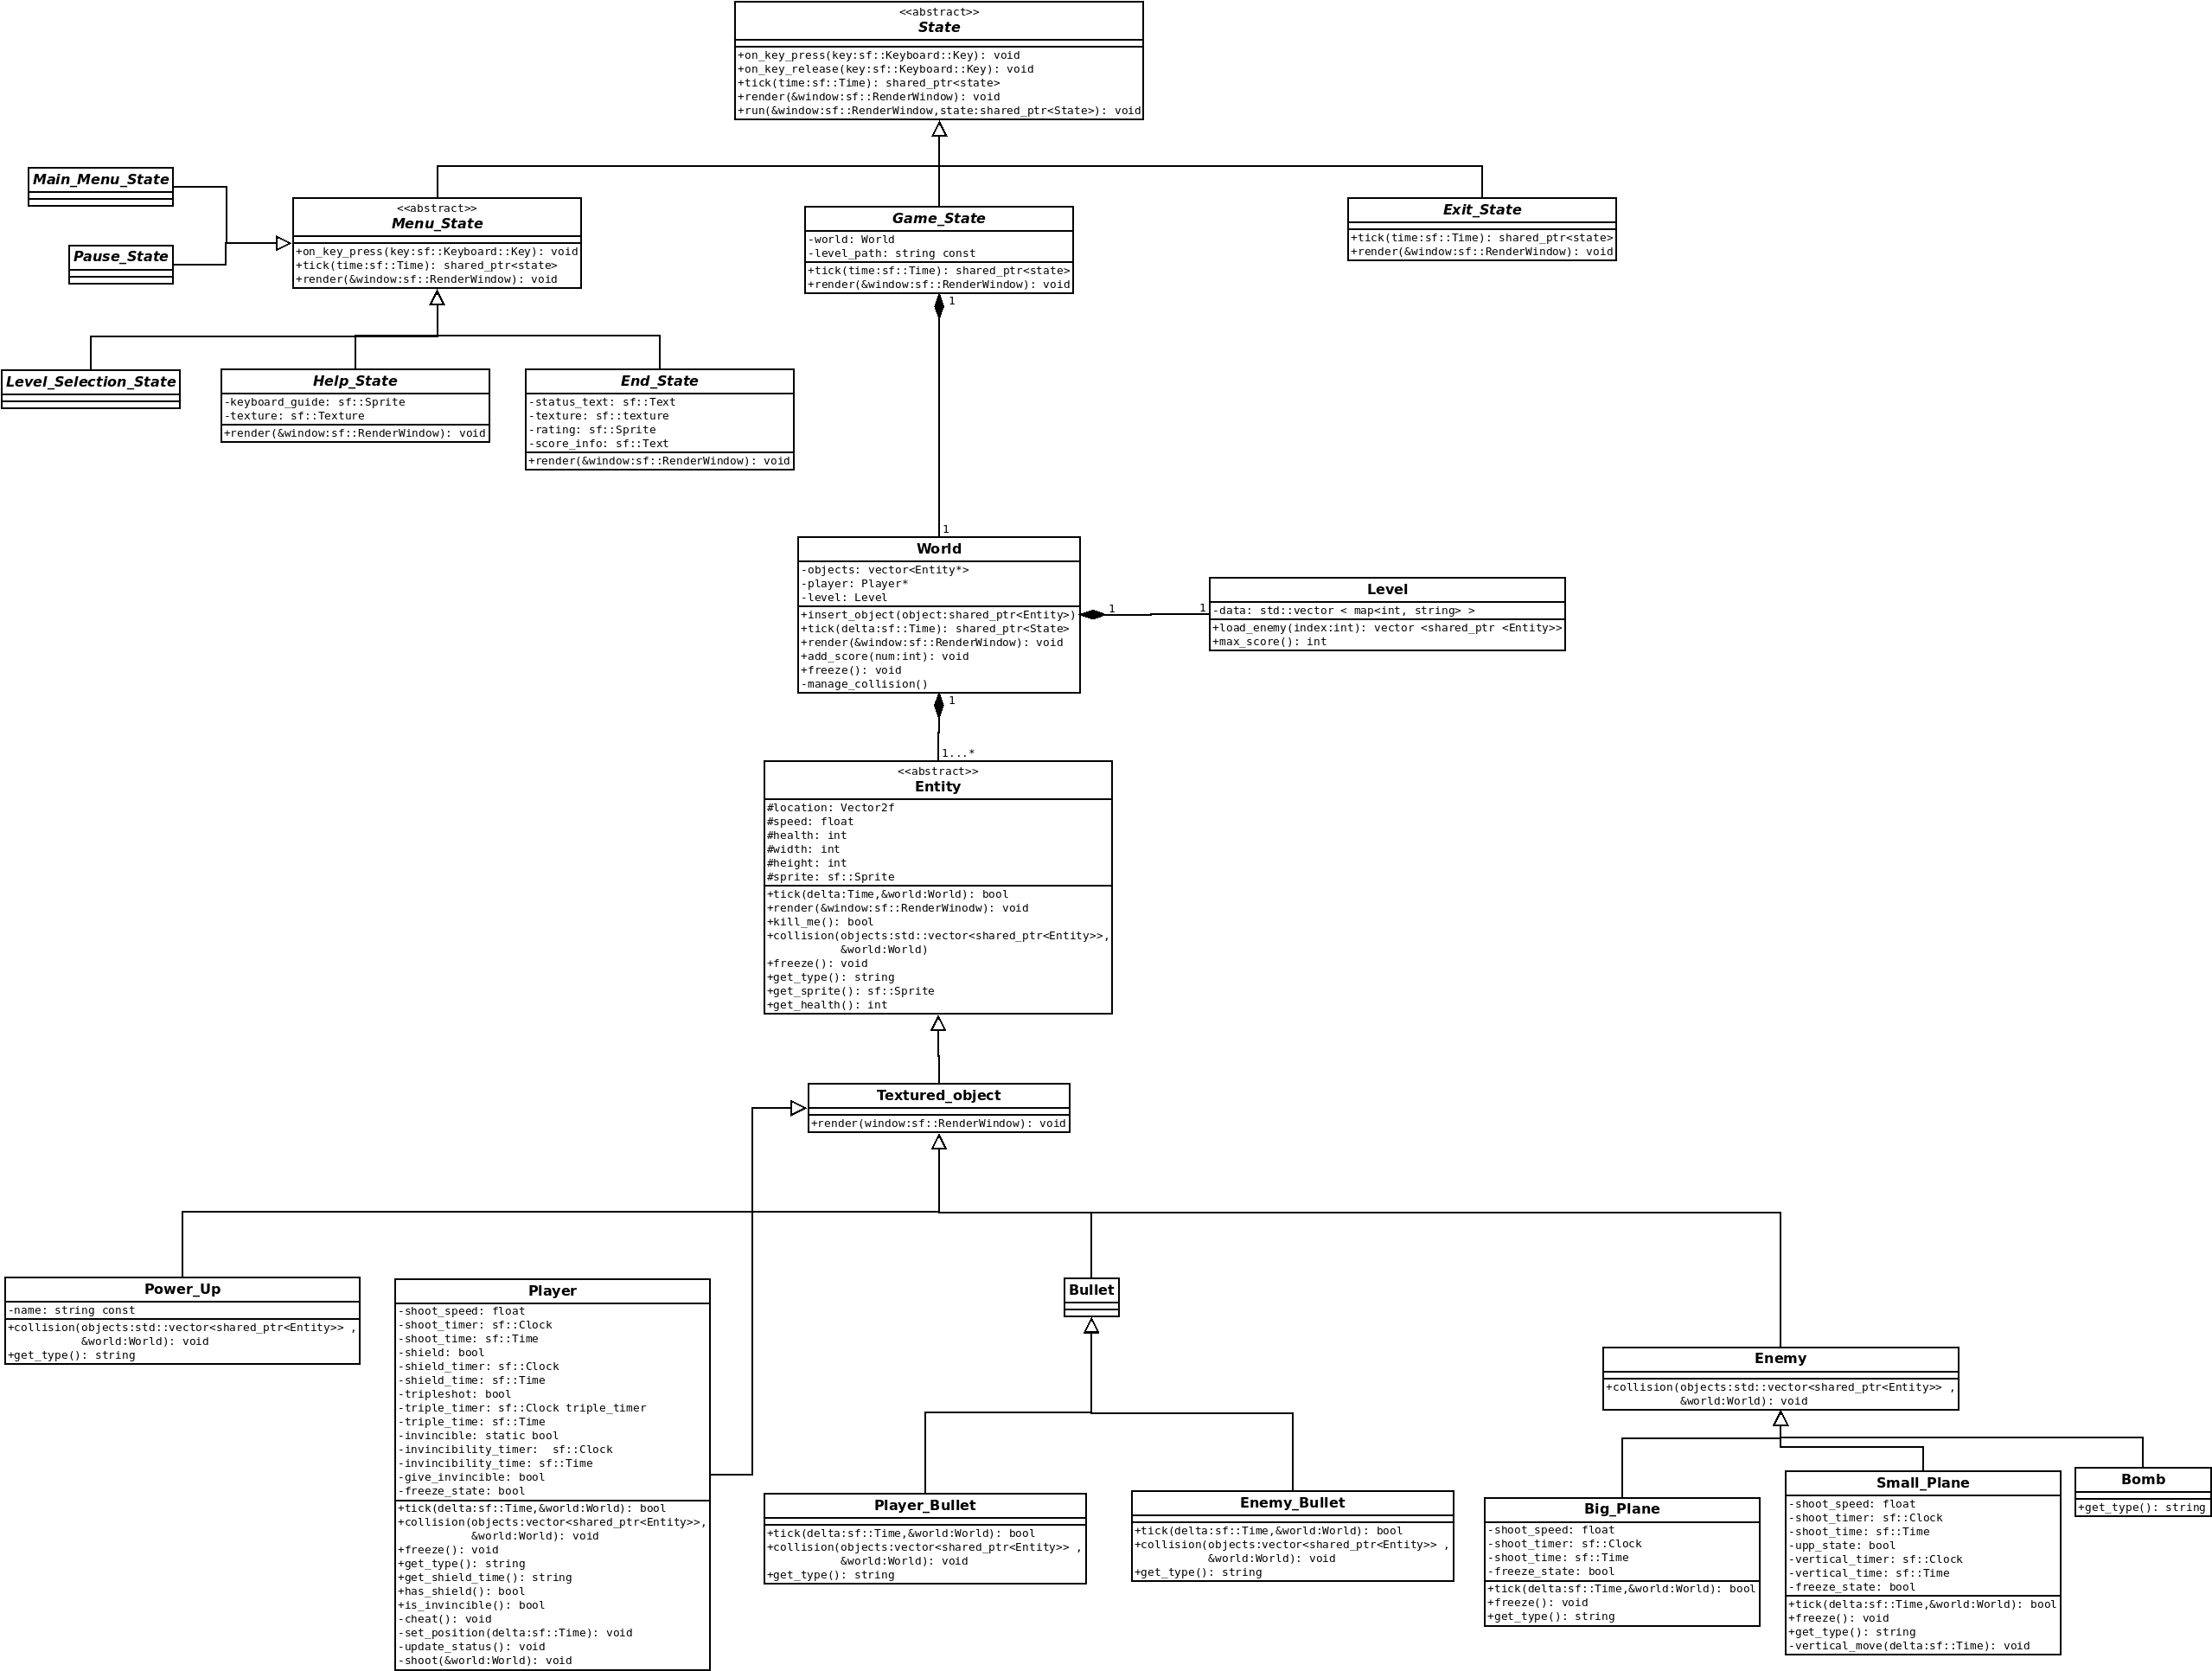
\includegraphics[scale=0.35]{UML_diagram.png}
\label{}
\caption{UML-diagram över spelet}
\end{figure}
\end{document}
